\chapter{Pętle}
Pętlą nazywamy instrukcję wielokrotnego wykonania tej samej czynności:
\begin{itemize}
\item określoną liczbę razy,
\item dla każdego elementu pewnego zbioru,
\item aż do spełnienia pewnego warunku,
\item w nieskończoność.
\end{itemize}

\section{Pętla FOR}
\begin{verbatim}
for ZMIENNA in ZBIÓR	
do	
  POLECENIA	
done
\end{verbatim}
\texttt{POLECENIA} zostaną wykonane tyle razy, ile elementów ma \texttt{ZBIÓR}, a \texttt{ZMIENNA} za każdym razem przyjmie kolejną wartość ze \texttt{ZBIORU}. \texttt{do} i \texttt{done} to klamry ograniczające listę \texttt{POLECEŃ} należących do pętli. Na przykład kod:
\begin{verbatim}
for i in "abc" "def" "ghi"	
do	
  echo $i	
done
\end{verbatim}
jest de facto równoważny kodowi:
\begin{verbatim}
echo "abc"	
echo "def"	
echo "ghi"
\end{verbatim}
Możemy pominąć \texttt{‘in ZBIÓR’}, wówczas zbiorem będą parametry skryptu. Następujący kod wyświetli na ekranie wszystkie parametry:
\begin{verbatim}
for i	
do	
  echo $i	
done	
\end{verbatim}

\subsection{Składnia ,,C-podobna''}
\begin{figure}[h!]
\centering
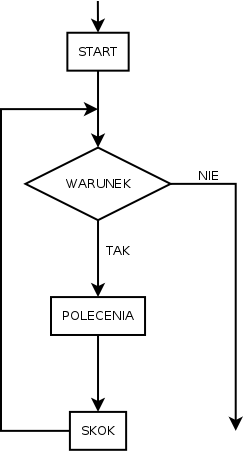
\includegraphics[width=3cm]{./ChA_5/for_diag.png}
\caption{Schemat blokowy pętli FOR}
\end{figure}
\FloatBarrier
%TODO if possible, use tikz to draw flowcharts - the one below is not good enough

%\begin{tikzpicture}[node distance = 2cm, auto]
%\node [point] (in) {};
%\node [block, below of=in] (start) {START};
%\node [decision, below of=start] (decide) {WARUNEK};
%\node [block, below of=decide] (instructions) {POLECENIA};
%\node [block, below of=instructions] (step) {SKOK};
%\node [point, right of=step, node distance=3cm] (out) {};
%
%\path [line] (in) -- (start);
%\path [line] (start) -- (decide);
%\path [line] (decide) -- (instructions);
%\path [line] (instructions) -- (step);
%\path [line] (step) -| ([xshift=-0.5cm]decide.west) -| ([xshift=-0.5cm]start.west) -| (start.west);
%\path [line] (decide) -| node [near start] {Nie} (out);
%\end{tikzpicture}

Inną składnią pętli for jest następująca:
\begin{verbatim}
for ((START ; WARUNEK ; SKOK))	
do	
  POLECENIA	
done
\end{verbatim}
Na początku zostanie wykonane polecenie \texttt{START}. Następnie będą powtarzane \texttt{POLECENIA} tak długo, jak długo jest spełniony \texttt{WARUNEK}. Po każdej iteracji będzie następował \texttt{SKOK}.\\

Powyższy kod wyświetli na ekranie:
\begin{verbatim}
1 2 3 4 5 6 7 8 9 10
\end{verbatim}
Zmiennej i najpierw zostanie przypisana wartość 1. Potem tak długo będzie ona wyświetlana i zwiększana o jeden, aż osiągnie wartość 10.\\

Przykładowo, aby wypisać na ekranie tabliczkę mnożenia możemy stworzyć następujący skrypt:
\begin{verbatim}
for ((i=1 ; i<=10 ; i++))	
do	
  for j in 1 2 3 4 5 6 7 8 9 10	
  do	
    echo "$i * $j = $((i*j))"	
  done	
done
\end{verbatim}
Zagnieżdżono jedną pętlę w drugiej. Obie robią to samo – wyliczają liczby naturalne od 1 do 10 – na różne sposoby. Po wykonaniu kodu otrzymamy sto linijek (10*10), wyglądające podobnie do: \texttt{7 * 8 = 56}.

\section{Pętla WHILE}
\begin{verbatim}
while [ WARUNEK ]	
do	
  POLECENIA	
done
\end{verbatim}
Pętla ta najpierw sprawdzi, czy \texttt{WARUNEK} jest prawdziwy, a jeśli tak, wykona \texttt{POLECENIA} i wróci do początku.\\
\begin{figure}[h!]
\centering
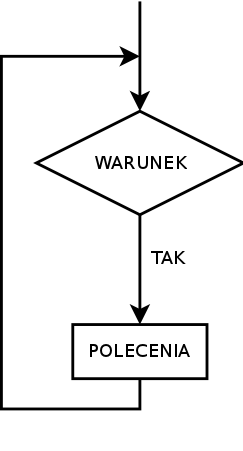
\includegraphics[width=3cm]{./ChA_5/while_diag.png}
\caption{Schemat blokowy pętli WHILE}
\end{figure}
\FloatBarrier
Przykładowa pętla wyliczająca liczby od 1 do 10 będzie wyglądała następująco:
\begin{verbatim}
i=1	
while [ $i –le 10 ]	
do	
  echo $i	
  i++	
done
\end{verbatim}

\section{Pętla UNTIL}
\begin{verbatim}
until [ WARUNEK ]	
do	
  POLECENIA	
done
\end{verbatim}
Konstrukcja ta różni się od while jedynie tym, że \texttt{WARUNEK} jest sprawdzany dopiero po, a nie przed, wykonaniem \texttt{POLECEŃ}. Oznacza to, że każda \texttt{until} wykona się co najmniej raz – dopiero potem sprawdzi, czy ma wrócić do początku, czy nie.\\
\begin{figure}[h!]
\centering
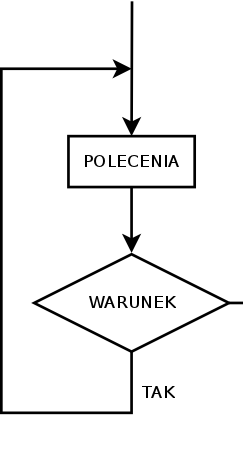
\includegraphics[width=3cm]{./ChA_5/until_diag.png}
\caption{Schemat blokowy pętli UNTIL}
\end{figure}
\FloatBarrier

\section{Pętle nieskończone}
Pętle, których \texttt{WARUNEK} nigdy nie zostanie spełniony będą wykonywać się w nieskończoność. Należy na to uważać, gdyż błędy nieskończonych pętli prowadzą do zawieszenia programu. 
\begin{verbatim}
i=1	
while [ $i –le 10 ]	
do	
  echo $i	
  i--	
done
\end{verbatim}
Zmienna \texttt{i} będzie zmniejszana aż do czasu, gdy przestanie być mniejsza od dziesięciu. Łatwo widać, że taka sytuacja nigdy nie nastąpi.\\

Nieskończona pętla nie musi jednak być błędem, a jest czasem zamierzonym działaniem programisty. Na przykład cały program \texttt{ping} znajduje się wewnątrz takiej pętli – będzie on pingował określony adres tak długo, aż użytkownik nie przerwie jego działania (\texttt{Ctrl+C}).

\section{Rekurencja}
Rekurencją nazywamy odwoływanie się funkcji do samej siebie. Taką sytuację można uznać za szczególny rodzaj pętli. Sztandarowym przykładem funkcji rekurencyjnej jest silnia.\\

\begin{math}
n! = \left\{
\begin{array}{l l}
1 & \quad dla n = 0 \\
n\ast(n-1)! & \quad dla n > 0 \\
\end{array}
\right.
\end{math}\\

\begin{itemize}
\item[] Aby policzyć 4! należy pomnożyć 4 przez 3!
\item[] Aby policzyć 3! należy pomnożyć 3 przez 2!
\item[] Aby policzyć 2! należy pomnożyć 2 przez 1!
\item[] Aby policzyć 1! należy pomnożyć 1 przez 0!
\item[] 0! jest dane – równe 1
\end{itemize}